% Every number in this paper is generated from frozen, hash-pinned artifacts
% listed in the repository's results summaries (docs/*.md). \pending{...}
% marks items still to be supplied by the author.
\documentclass[11pt]{article}
\usepackage[preprint]{acl}
\usepackage{times}
\usepackage{latexsym}
\usepackage[T1]{fontenc}
\usepackage[utf8]{inputenc}
\usepackage{microtype}
\usepackage{inconsolata}
\usepackage{graphicx}
\usepackage{booktabs}
\usepackage{amsmath,amssymb}
\usepackage{xcolor}
\usepackage{algorithm}
\usepackage{algpseudocode}

% Numbered citations, [1], [2], ... (references sorted by author, as
% acl_natbib.bst orders them). Set to \numberedcitationsfalse for the ACL
% author-year style.
\newif\ifnumberedcitations
\numberedcitationstrue
\ifnumberedcitations
  \setcitestyle{numbers,square,comma}
\fi

\newcommand{\pending}[1]{\textcolor{red}{[#1]}}
\newcommand{\Rstop}{R_{\mathrm{stop}}}
\newcommand{\CM}{C_{M}}
\newcommand{\CFA}{C_{FA}}
\newcommand{\Cr}{C_{r}}

\title{Direct Density Ratio Estimation for Efficient Retriever-aware\\
Hallucination Detection in Large Language Models}

\author{Augustine Manu-Frimpong \\
  Grambling State University \\
  \texttt{afrimpon@gsumail.gram.edu}}

\begin{document}
\maketitle

\begin{abstract}
Retrieval-based hallucination detectors verify LLM claims against evidence
documents, and every document read costs NLI calls. Bayesian sequential
estimation (BSE) reads documents one at a time and stops when another is not
worth its cost. It weighs each document by a likelihood ratio that it obtains
by counting two histograms of entailment scores and dividing them. We keep
BSE's pipeline fixed and change only this step: the ratio is estimated
directly by density-ratio estimation (uLSIF). Along the way we find that
BSE's published one-step look-ahead, implemented as written, never reads a
document at the published costs. We therefore stop every method by backward
induction, which we derive for any ratio estimator. In a preregistered test
on HELM (3,736 sentences from seven LLMs), the direct ratio's cost--quality
curve lies above BSE's at both published cost settings (area gap +0.043 and
+0.037 balanced AP). At BSE's quality it needs 2.7 fewer NLI calls per
sentence (70\% fewer). Its curve also lies above a simple fixed-$k$ maximum-entailment
baseline, which BSE's does not. A retriever-aware multivariate variant is
not supported. Effects are modest but consistent across five exploratory
datasets and the confirmatory test.
\end{abstract}

\section{Introduction}

LLMs produce fluent text that is sometimes false. A common way to detect such
hallucinations is to split a sentence into claims, retrieve evidence for each
claim, and score claim--evidence pairs with a natural-language-inference (NLI)
model \citep{min-etal-2023-factscore,wang-etal-2024-factcheck}. The cost of
such detectors grows with every document they read. This matters most in
deployed assistants that check responses before they reach users, for example
customer-service systems in enterprises. There, every retrieved and scored
document adds compute and latency to each response, so a detector that
reaches the same reliability with fewer documents is directly cheaper to
run.

\citet{wang-etal-2023-hallucination} cast this as Bayesian sequential
estimation (BSE). Documents are read in retrieval order. After each one, the
posterior probability that the claim is factual is updated, and a Bayes-risk
rule decides whether reading another document is worth its cost
\citep{wald1945sequential}.

The quality and the cost of this process both hinge on one quantity: the
likelihood ratio that turns a document's entailment score into evidence.
BSE estimates it by counting two 10-bin histograms, one for factual and one
for hallucinated claims, and dividing them. The density-ratio literature
warns against exactly this two-step route. Estimating each density separately
is harder than estimating their ratio, and dividing amplifies both errors
\citep{sugiyama2012density}.

We ask whether estimating the ratio \emph{directly} makes sequential
hallucination detection cheaper and better, with everything else held fixed.
Our goals are:
\begin{itemize}
\item \textbf{G1 (cost):} reach BSE's detection quality with fewer NLI calls;
\item \textbf{G2 (detection):} detect hallucinations better at BSE's cost;
\item \textbf{G3 (calibration):} give better-calibrated probabilities.
\end{itemize}

\paragraph{Contributions.}
\begin{enumerate}
\item A drop-in replacement of BSE's likelihood ratio by direct density-ratio
estimation, uLSIF \citep{kanamori2009ulsif}. The documents, prior,
update, stopping rule and aggregation are all unchanged (\S\ref{sec:method}).
\item A finding about BSE's stopping rule. The published one-step look-ahead,
implemented as written, never reads a document at the published costs,
because no single document can flip the decision from the prior.
\begin{itemize}
\item We show that the look-ahead's expectation can be computed for
\emph{any} ratio estimator from its own training sample.
\item We use this to stop every method by backward induction, the
Bayes-optimal rule BSE's authors name but approximate
(\S\ref{sec:stopping}).
\end{itemize}
\item A preregistered confirmatory test on a dataset no detector of ours had
touched. The direct ratio's cost--quality curve lies above BSE's and above
a simple fixed-$k$ baseline (\S\ref{sec:helm}).
\item Negative results reported in full:
\begin{itemize}
\item a retriever-aware multivariate ratio does not beat its histogram
control;
\item BSE lies below the fixed-$k$ baseline;
\item earlier configurations did not survive testing (\S\ref{sec:negative}).
\end{itemize}
\end{enumerate}

\section{Background: Bayesian sequential estimation}
\label{sec:bse}

\paragraph{Scoring and update.} For a claim $c$ and its ranked documents
$d_1, d_2, \dots$, an NLI model gives each document an entailment score
$e \in [0, 100]$: the maximum entailment probability over 400-word spans,
with softmax temperature 5. Starting from prior $\pi_0 = 0.5$, BSE updates
the probability that $c$ is factual after each document:
\begin{equation}
\pi' = \frac{\pi\, r(e)}{\pi\, r(e) + 1 - \pi},
\label{eq:update}
\end{equation}
where $r(e) = p(e \mid \text{factual}) / p(e \mid \text{hallucinated})$.
BSE estimates $r$ as the ratio of two Laplace-smoothed 10-bin histograms of
$e$, counted over 199 factual and 199 hallucinated claim--document pairs.

\paragraph{Stopping.} With miss cost $\CM$, false-alarm cost $\CFA$ and
retrieval cost $\Cr$, the risk of stopping is
$\Rstop(\pi) = \min\{(1-\pi)\CM,\ \pi\CFA\}$. BSE's Eq.~8 continues iff
$\Rstop(\pi) > \Cr + \mathbb{E}_{\text{next}}[\Rstop(\pi')]$, a one-step
look-ahead \citep{cardillo1968suboptimal}.

\paragraph{Decision.} A sentence's probability is the minimum over its
claims. The sentence is labelled factual iff $(1-\pi)\CM < \pi\CFA$.

\paragraph{Paper vs released code.} BSE's released code differs from the
paper in 26 documented details. For example:
\begin{itemize}
\item spans are 400 \emph{words} with a stride of 300;
\item the look-ahead averages the ten possible next posteriors with uniform
weights, instead of weighting them by predictive probability.
\end{itemize}
Our reproduction follows the code, and matches the published Table~1 at
$\CM{=}28$, $\CFA{=}96$. Our repository tabulates every difference.

\section{Direct density-ratio evidence}
\label{sec:method}

Eq.~\ref{eq:update} needs only the ratio $r$, never the two densities.

\paragraph{BSE's ratio, for contrast.} BSE discretises $e$ into ten bins
$b(e)$, counts the $N_f$ factual and $N_h$ hallucinated training pairs per
bin ($n_f(b)$, $n_h(b)$) and divides the two smoothed histograms:
\begin{equation}
r_{\mathrm{BSE}}(e) = \frac{\bigl(n_f(b(e)) + 1\bigr) / (N_f + 10)}
                           {\bigl(n_h(b(e)) + 1\bigr) / (N_h + 10)}.
\label{eq:bse-ratio}
\end{equation}

\paragraph{Direct estimation (uLSIF).} Instead, we fit the ratio itself
with unconstrained least-squares importance fitting
\citep{kanamori2009ulsif}. Let $x^f_1, \dots, x^f_{n_f}$ be the features of
documents of factual claims and $x^h_1, \dots, x^h_{n_h}$ those of
hallucinated claims, standardised on the pooled sample. The model is a
non-negative combination of Gaussian kernels on $L = 100$ centres $c_l$
drawn from the factual sample:
\begin{equation}
\hat r(x) = \sum_{l=1}^{L} \alpha_l \exp\!\Bigl(-\frac{\lVert x - c_l\rVert^2}{2\sigma^2}\Bigr).
\label{eq:ulsif-model}
\end{equation}
uLSIF minimises the squared error
$\tfrac12 \mathbb{E}_h[(\hat r - r)^2]$, which up to a constant equals
$\tfrac12 \mathbb{E}_h[\hat r^2] - \mathbb{E}_f[\hat r]$. With a ridge
penalty, the empirical objective is
\begin{equation}
\min_{\alpha}\ \tfrac12\, \alpha^\top \hat H \alpha - \hat h^\top \alpha
  + \tfrac{\lambda}{2}\, \alpha^\top \alpha,
\label{eq:ulsif-objective}
\end{equation}
where $\hat H_{ll'} = \frac{1}{n_h}\sum_j k_l(x^h_j)\, k_{l'}(x^h_j)$,
$\hat h_l = \frac{1}{n_f}\sum_i k_l(x^f_i)$ and $k_l$ is the $l$-th kernel.
Its solution is in closed form, with negative weights set to zero:
\begin{equation}
\hat\alpha = \max\bigl\{0,\ (\hat H + \lambda I)^{-1} \hat h\bigr\}.
\label{eq:ulsif-solution}
\end{equation}

\paragraph{Model selection.} The kernel width $\sigma$
($0.125$--$4\times$ the median pairwise distance) and $\lambda$
($10^{-4}$--$10$) minimise the held-out criterion
\begin{equation}
J(\sigma, \lambda) = \tfrac12\, \overline{\hat r(x^h)^2}
  - \overline{\hat r(x^f)}
\label{eq:ulsif-cv}
\end{equation}
over five folds, where the bars average over held-out documents. Folds are
grouped by claim, so that documents of one claim never straddle folds. No
detection metric is used.

\paragraph{Self-normalisation.} A ratio should average 1 under the
hallucinated distribution, $\mathbb{E}_h[r] = 1$. uLSIF's fit need not, which
biases every update. We therefore use
\begin{equation}
\tilde r(x) = \hat r(x) \Big/ \frac{1}{n_h}\sum_{j=1}^{n_h} \hat r(x^h_j),
\label{eq:normalise}
\end{equation}
clipped to $[10^{-6}, 10^{6}]$. In the update, Eq.~\ref{eq:update}, the
ratio $r(e)$ is replaced by $\tilde r(x)$.

\paragraph{Estimators compared.} The pure test, \textbf{DDRE-1D}, fits
$\hat r(e)$ on exactly BSE's 398 training pairs. Against BSE it changes only
how the ratio is estimated.

As a retriever-aware variant, \textbf{DDRE-M} uses three features per
document: entailment, contradiction (from the same NLI pass) and log
retrieval rank. Its control, \textbf{NB-M}, multiplies per-feature
histograms (Naive Bayes) on the same features. Both are fitted on an
entity-disjoint split of FActScore \citep{min-etal-2023-factscore}: 7,382
facts, each with 10 BM25-retrieved Wikipedia passages.

\section{Stopping by backward induction}
\label{sec:stopping}

\paragraph{The one-step rule never reads.} At $\CM{=}28$, $\CFA{=}96$, the
prior $\pi_0 = 0.5$ already sits on the ``factual'' side of the decision
threshold $28/124 = 0.226$. Flipping the decision requires a log ratio below
$\operatorname{logit}(0.226) = -1.23$. The strongest negative bin of BSE's
histogram has $\log r = -0.69$. So no single document can change the
decision, and the one-step value of reading one is exactly zero.

Eq.~8 therefore never reads, for any $\Cr > 0$; two independent
implementations agree. BSE's released code instead takes the stop risk of the
unweighted mean of the ten next posteriors. That gives a continue region of
$(0.204, 0.769)$, which is why the published system reads documents at all.

\paragraph{The look-ahead for any ratio estimator.} The expectation in Eq.~8
is over the next document's features under the predictive mixture
$\pi p_f + (1-\pi) p_h$. Since $p_f = r\, p_h$,
\begin{equation}
\mathbb{E}_{\text{next}}[g] = \mathbb{E}_{h}\!\left[(\pi r(x) + 1 - \pi)\, g(\pi')\right],
\label{eq:identity}
\end{equation}
which needs only the estimator's ratio and its own hallucinated training
sample. For $g = \Rstop$ the weight cancels the posterior's denominator:
$(\pi r + 1 - \pi)\Rstop(\pi') = \min\{(1-\pi)\CM,\ \pi r \CFA\}$.
\begin{itemize}
\item For BSE's histogram, Eq.~\ref{eq:identity} reproduces Eq.~8 exactly.
\item For DDRE it gives the same rule, with no borrowed thresholds.
\end{itemize}

\paragraph{Backward induction.} With $n$ documents read and at most $K$
available, the optimal expected cost is
\begin{equation}
V_n(\pi) = \min\{\Rstop(\pi),\ \Cr + \mathbb{E}_{\text{next}}[V_{n+1}(\pi')]\},
\end{equation}
with $V_K = \Rstop$.
\begin{itemize}
\item BSE's authors describe this as the optimal solution, but approximate
it, because induction over discrete features grows exponentially.
\item Our state is the scalar posterior, so we solve it on a logit grid,
using Eq.~\ref{eq:identity} for the expectation.
\item With one document left, it equals Eq.~8.
\end{itemize}
Algorithm~\ref{alg:ddre} summarises the whole procedure.

\begin{algorithm}[t]
\caption{Sequential hallucination detection with a direct density-ratio
evidence model (DDRE).}
\label{alg:ddre}
\small
\begin{algorithmic}[1]
\Statex \textbf{Offline} (once per estimator)
\State Fit $\hat r$ by uLSIF (Eqs.~\ref{eq:ulsif-model}--\ref{eq:ulsif-solution}), choosing $(\sigma, \lambda)$ by Eq.~\ref{eq:ulsif-cv}
\State Self-normalise: $\tilde r \gets \hat r / \overline{\hat r(x^h)}$ (Eq.~\ref{eq:normalise})
\State Support $\mathcal{S} \gets \{\log \tilde r(x^h_j)\}_{j=1}^{n_h}$, the hallucinated training sample
\For{$n = K-1, \dots, 0$} \Comment{backward induction}
  \State $V_n(\pi) \gets \min\{\Rstop(\pi),\ \Cr + \mathbb{E}_{\text{next}}[V_{n+1}(\pi')]\}$, expectation by Eq.~\ref{eq:identity} over $\mathcal{S}$
\EndFor
\Statex \textbf{Online} (one claim $c$, ranked documents $d_1, \dots, d_K$)
\State $\pi \gets \pi_0$
\For{$n = 0, \dots, K-1$}
  \If{$\Rstop(\pi) \le \Cr + \mathbb{E}_{\text{next}}[V_{n+1}(\pi')]$} \textbf{break} \EndIf
  \State $x \gets$ NLI features of $(d_{n+1}, c)$ \Comment{one NLI pass per span}
  \State $\pi \gets \pi\, \tilde r(x) / \bigl(\pi\, \tilde r(x) + 1 - \pi\bigr)$ \Comment{Eq.~\ref{eq:update}}
\EndFor
\State \Return $\pi$; a sentence takes the minimum over its claims and is factual iff $(1-P)\CM < P\,\CFA$
\end{algorithmic}
\end{algorithm}

For BSE at $\CM{=}28$, $\CFA{=}96$, $\Cr{=}1$ and $K{=}10$ it continues while
$\pi \in (0.034, 0.813)$. Every method in our comparisons is stopped by this
rule, so they differ only in $r$.

\section{Evaluation protocol}
\label{sec:protocol}

\paragraph{Cost and quality.}
\begin{itemize}
\item \textbf{Cost:} NLI calls per sentence; documents per sentence is
reported too.
\item \textbf{Quality:} balanced average precision (AP), the mean of the AP
for the factual class and the AP for the hallucinated class.
\end{itemize}
We use AP rather than the trapezoidal PR-AUC of BSE's code for one reason.
On ties, the trapezoid rewards coarse scores. A constant score gets $0.75$
balanced trapezoidal PR-AUC but $0.5$ balanced AP, and BSE's histogram
posteriors are heavily tied.

\paragraph{Cost--quality curves.} Each method is run at every combination of
$K \in \{1,\dots,10\}$ (maximum documents per claim) and
$\Cr \in \{0.125, 0.25, 0.5, 1\}$, at both of BSE's cost settings, 28/96 and
14/24. Its curve is the step envelope of these operating points: the best AP
reachable within a given cost.
\begin{itemize}
\item \textbf{Primary endpoint:} the \emph{AUC-gap}, the mean AP difference
between two envelopes over their shared cost range.
\item \textbf{Cost saving (G1):} NLI calls saved at the reference method's AP.
\item \textbf{Quality gain (G2):} AP gained at the reference method's cost.
\end{itemize}

\paragraph{Baseline and statistics.}
\begin{itemize}
\item \textbf{Fixed-$k$ baseline:} read the first $k$ documents and take the
maximum entailment, BSE's own ``Maximum'' baseline.
\item \textbf{Intervals:} a paired cluster bootstrap (10,000 replicates)
resamples whole passages, entities, responses or articles. Every method is
evaluated on the same draws.
\end{itemize}

\paragraph{Exploratory vs confirmatory.} Five datasets had been used during
development, so results on them are \emph{exploratory}. These are the
SelfCheckGPT held-out split \citep{manakul-etal-2023-selfcheckgpt}, the
FActScore test entities, Factcheck-Bench \citep{wang-etal-2024-factcheck},
ExpertQA \citep{malaviya-etal-2024-expertqa} and BingCheck
\citep{li-etal-2024-self}.

The confirmatory test uses HELM \citep{su-etal-2024-unsupervised}. Its
hypotheses, endpoints and decision rule were merged as a preregistration
\citep{nosek2018preregistration} before any retrieval, NLI scoring or
detector touched it.

\section{Results}
\label{sec:results}

\subsection{Exploratory results (five used datasets)}

Table~\ref{tab:explore} gives the AUC-gaps.
\begin{itemize}
\item \textbf{DDRE-1D vs BSE:} the gap is positive on all five datasets at
both cost settings, and every interval excludes zero.
\item \textbf{Fixed-$k$:} BSE's envelope lies below the fixed-$k$ baseline on
four of five datasets at 28/96, while DDRE-1D's lies at or above it.
\item \textbf{Effect sizes} are small (at most 0.041 AP). ExpertQA carries
almost no signal for any method (AP $\approx 0.51$).
\end{itemize}

\begin{table}[t]
\centering\small
\setlength{\tabcolsep}{3pt}
\begin{tabular}{@{}lcccc@{}}
\toprule
 & \multicolumn{2}{c}{DDRE-1D $-$ BSE} & \multicolumn{2}{c}{DDRE-1D $-$ fixed-$k$} \\
Dataset & 28/96 & 14/24 & 28/96 & 14/24 \\
\midrule
SelfCheckGPT & \textbf{+.023} & \textbf{+.020} & \textbf{+.013} & \textbf{+.019} \\
FActScore & \textbf{+.031} & \textbf{+.026} & +.004 & \textbf{+.010} \\
Factcheck-B. & \textbf{+.041} & \textbf{+.035} & $-$.002 & \textbf{+.016} \\
ExpertQA & \textbf{+.003} & \textbf{+.004} & \textbf{+.003} & \textbf{+.002} \\
BingCheck & \textbf{+.012} & \textbf{+.013} & \textbf{+.010} & \textbf{+.016} \\
\bottomrule
\end{tabular}
\caption{Exploratory AUC-gaps in balanced AP. Bold: the 95\% cluster-bootstrap
interval excludes 0.}
\label{tab:explore}
\end{table}

\subsection{Preregistered confirmatory test on HELM}
\label{sec:helm}

\paragraph{Data.} HELM has 3,736 sentences continuing Wikipedia articles,
1,978 of them hallucinated, from seven LLMs. Two annotators labelled each
sentence. The sentences come from 229 articles, which are the bootstrap
clusters.

\paragraph{Protocol.}
\begin{itemize}
\item \textbf{Units:} each sentence is a single claim; HELM releases no
decompositions.
\item \textbf{Evidence:} the top 10 BM25 passages from a 2023 Wikipedia
snapshot, with the article title and the sentence as the query.
\item \textbf{Hypotheses:} H1, DDRE-1D's curve lies above BSE's; H2, it lies
above the fixed-$k$ baseline's.
\item \textbf{Decision rule:} each is tested at both cost settings, with
Holm's correction \citep{holm1979simple} over the four one-sided tests.
\end{itemize}

\begin{table}[t]
\centering\small
\setlength{\tabcolsep}{3pt}
\begin{tabular}{@{}llccc@{}}
\toprule
Test & $\CM/\CFA$ & AUC-gap & 5th pct. & $p$ \\
\midrule
H1a: vs BSE & 28/96 & \textbf{+0.043} & +0.036 & $<10^{-4}$ \\
H1b: vs BSE & 14/24 & \textbf{+0.037} & +0.030 & $<10^{-4}$ \\
H2a: vs fixed-$k$ & 28/96 & \textbf{+0.008} & +0.002 & 0.012 \\
H2b: vs fixed-$k$ & 14/24 & \textbf{+0.016} & +0.010 & $<10^{-4}$ \\
\bottomrule
\end{tabular}
\caption{Preregistered test on HELM: DDRE-1D against BSE and against fixed-$k$
maximum entailment. One-sided cluster-bootstrap $p$ (10,000 replicates over
229 articles). All four are supported after Holm's correction.}
\label{tab:helm}
\end{table}

\begin{figure}[t]
\centering
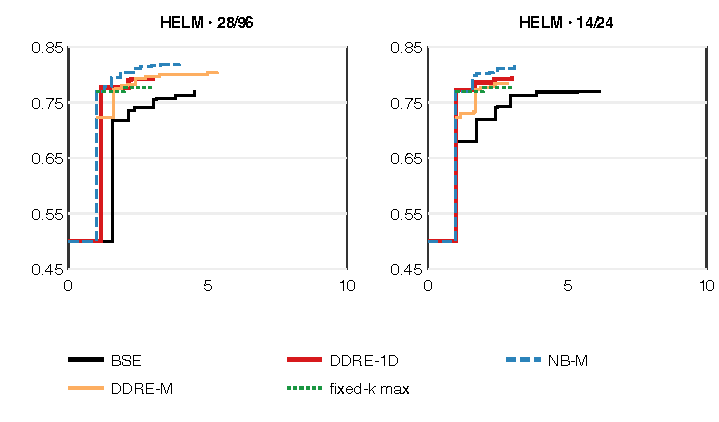
\includegraphics[width=\columnwidth]{figures/helm_envelopes.pdf}
\caption{HELM cost--quality envelopes (balanced AP against NLI calls per
sentence) over all $(K, \Cr)$ operating points.}
\label{fig:helm}
\end{figure}

\paragraph{Decision.} Both hypotheses are confirmed (Table~\ref{tab:helm},
Figure~\ref{fig:helm}).

\paragraph{Secondary endpoints, at 28/96 unless stated.}
\begin{itemize}
\item \textbf{G1 (cost):} at BSE's AP, DDRE-1D needs 2.68 fewer NLI calls per
sentence (95\% CI [1.86, 3.49]); 1.43 [0.72, 1.48] fewer at 14/24. BSE's
cheapest operating point that reaches that AP needs 3.85 calls (2.43 at
14/24), against DDRE-1D's 1.16 (1.00), i.e.\ 70\% (59\%) fewer.
\item \textbf{G2 (detection):} at BSE's cost, its AP is higher by +0.024
[0.016, 0.036]; by +0.035 [0.025, 0.046] at 14/24.
\item \textbf{G3 (calibration):} its Brier score is lower at both operating
points (0.213 vs.\ 0.233; 0.198 vs.\ 0.211).
\end{itemize}

\paragraph{Robustness.}
\begin{itemize}
\item \textbf{H1:} it holds when passages from the source article (22\% of
the evidence) are removed, on the six generators described by HELM's
authors, and for each of the seven generators separately (+0.026 to +0.051).
\item \textbf{H2:} it is narrower. At 28/96 it is not supported on the
six-generator subset, and two of seven generators are slightly negative
there.
\end{itemize}

\paragraph{Where the advantage lies.} At BSE's operating point itself
($K{=}10$, $\Cr{=}1$), DDRE-1D reads slightly more (5.87 vs.\ 5.46 NLI calls)
for slightly higher AP (0.766 vs.\ 0.762). Its advantage is in reaching a
given quality more cheaply along the curve.

\subsection{What did not work}
\label{sec:negative}

\paragraph{Retriever-aware DDRE.} DDRE-M lies below its histogram control
NB-M on HELM (AUC-gap $-0.024$ and $-0.033$) and on most exploratory
datasets. Adding contradiction and rank helps the histogram estimator: NB-M
has the highest AP on HELM. It does not help uLSIF. So we do not support the
retriever-aware variant.

\paragraph{BSE vs.\ the simple baseline.} BSE's envelope lies below fixed-$k$
maximum entailment on HELM ($-0.041$ and $-0.028$) and on most exploratory
datasets.

\paragraph{Earlier configurations.} Before the single-factor design above,
two configurations failed:
\begin{itemize}
\item a 1-D DDRE whose stopping band and kernel width were tuned over 640
validation configurations;
\item a multivariate DDRE run under BSE's stopping band.
\end{itemize}
They gave cost or quality gains on single datasets. Neither transferred, and
the second was not confirmed by a preregistered test on ExpertQA and
BingCheck. Both differed from BSE in more than the likelihood ratio. All
are reported in the repository.

\section{Related work}

\paragraph{Hallucination detection.}
\begin{itemize}
\item \textbf{Sampling-based:} SelfCheckGPT
\citep{manakul-etal-2023-selfcheckgpt} compares sampled generations.
\item \textbf{Retrieval-based:} FActScore and Factcheck-GPT score atomic
claims against retrieved evidence
\citep{min-etal-2023-factscore,wang-etal-2024-factcheck,wei2024longform}.
\item \textbf{Internal-state:} MIND and HELM use the model's own internal
states \citep{su-etal-2024-unsupervised}.
\end{itemize}
BSE \citep{wang-etal-2023-hallucination} is, to our knowledge, the only one
that decides adaptively how many documents to read. We change its evidence
model and its stopping computation.
See \citet{ji2023survey} for a survey.

\paragraph{Sequential decisions.} Sequential analysis
\citep{wald1945sequential} and one-step approximations to Bayesian stopping
\citep{cardillo1968suboptimal} underlie BSE. Our backward induction is the
exact finite-horizon solution for a scalar posterior.

\paragraph{Density-ratio estimation.}
\begin{itemize}
\item \textbf{Direct estimators:} KLIEP \citep{sugiyama2007kliep}, uLSIF
\citep{kanamori2009ulsif}, RuLSIF \citep{yamada2011rulsif} and
probabilistic classification \citep{bickel2009discriminative}.
\item \textbf{Unified view:} these are instances of density-ratio matching
under a Bregman divergence \citep{sugiyama2012bregman,sugiyama2012density}.
\end{itemize}
They are used for covariate shift, two-sample tests and outlier detection.
Using them as the evidence model of a sequential detector is, to our
knowledge, new.

\section{Discussion}

\paragraph{What the results support.} A directly estimated likelihood ratio
improves BSE's cost--quality trade-off, and the effect replicated under a
preregistered test. The gain in quality is modest, about 0.04 AP across the curve. The cost
saving at equal quality is larger: 70\% fewer NLI calls than BSE on HELM at
28/96, from 3.85 to 1.16 per sentence.

\paragraph{Why curves, not one operating point.} A better-estimated ratio
does not, by itself, shorten the walk to a fixed stopping region. Its benefit
shows when cost is allowed to vary, so evaluations of sequential detectors
should report curves, not a single operating point.

\paragraph{Implications for deployment.} In retrieval-augmented
assistants, such as enterprise customer-service systems, NLI scoring of
retrieved evidence dominates a detector's per-response compute. The
estimator itself costs little: a histogram lookup, or a kernel sum over 100
centres. At equal detection quality, the direct ratio needed 70\% fewer NLI
calls than BSE on HELM. That suggests a proportional saving in verification
compute for such systems.

We did not test this setting. Domain-specific knowledge bases, different
retrievers and the cost of a wrong answer in customer service may change both
the size of the saving and the best operating point. A measured evaluation on
customer-service data, with wall-clock latency, is the natural next step.

\paragraph{Lessons for evaluation.}
\begin{itemize}
\item A competitive simple baseline (fixed-$k$ maximum entailment) should
always be included; BSE does not beat it.
\item The stopping rule needs care. BSE's published Eq.~8 is degenerate at
its own costs, while its code works by a heuristic.
\end{itemize}

\section*{Limitations}

\begin{itemize}
\item \textbf{Effect sizes} are small, and H2 at 28/96 is narrow.
\item \textbf{Exploratory datasets:} five datasets were used during
development. Only HELM is confirmatory.
\item \textbf{Protocol differences:} on HELM, evidence comes from our own
BM25 retrieval over a Wikipedia snapshot, not live web search. Sentences are
not decomposed into claims.
\item \textbf{HELM labels:}
\begin{itemize}
\item annotators also consulted Google;
\item the handling of ``unverifiable'' sentences in the binary labels is
undocumented;
\item the released counts differ from the paper's;
\item no licence is stated.
\end{itemize}
We contacted the authors on 17 October 2026.
\item \textbf{Training mismatch:} BSE and DDRE-1D are fitted on BSE's 398
training pairs. These pairs are scored on whole premises, while test
documents are scored as the maximum over spans. Both methods inherit this
mismatch.
\item \textbf{Application domain:} we evaluated on general-domain and
Wikipedia-grounded data only, not on enterprise or customer-service data.
\item \textbf{Cost} is counted in NLI calls and documents. We did not
measure wall-clock time; estimator overhead is small next to the NLI model
but unmeasured.
\end{itemize}

\section*{Reproducibility}

Code, preregistrations, amendments, decision records and results summaries are
in the repository \pending{URL}. Every artifact is identified by its SHA-256
digest, and every run was made once from a reviewed commit. No dataset is
redistributed.

\bibliography{refs}

\end{document}
